\chapter{Discussion}
\label{Discussion}

In phase 2 of the study, we found that our high severity tiered warning messages outperformed Firefox's control warnings in terms of adherence rates, user reaction times, and user perceptions of severity. In this section, we will discuss possible reasons for these results, some other incidental findings from the study, and the overall implications.


\section{Phase 1}
Unfortunately, due to limited time and resources we were not able to collect enough data in phase 1 of the study to draw any statistically supported conclusions. Participants were debriefed after being presented with deceptive warning message. This means that each participant only saw one warning in this phase which consequently resulted in a very small sample size. However, behaviour during this phase should not be completely ignored as it provides some rough insight into user habits in a more ecologically valid scenario (no participants reported that they were aware of the deception used in phase 1). It also confirms the findings of previous studies.

Participants in phase 1 generally ignored the warning fairly quickly. Eye tracking data shows that many alternated between looking at the ``go back'' and ``ignore warning'' buttons repeatedly in apparent hesitation before making their final decision. It was also common for participants to fixate on a warning's title and skim or not read the body of the message (although some did). Both of these occurrences suggest to us that participants were trying to decide simply between visiting the website or not, rather than evaluating the type of risk the warning presented them with. The warning was merely acting as a roadblock in the way of their regular browsing -- a nuisance. Some expressed their disregard in the subsequent questionnaire with responses such as ``I didn't really pay attention to [the warning]'' and ``[The warning] was not difficult to read, but I should have read it slower''. This behaviour was seen for both the control messages and our tiered messages and is consistent with habituation effects and warning fatigue that have been previously observed by others \cite{akhawe2013alice, anderson2015polymorphic, egelman2008warned}.

\subsection{Perceived Risk}
We hypothesized that participants would be more likely to consider a warning message if they believed that personal information was at risk. We attempted to accomplish this in phase 1 by asking participants to sign into their university email account to view a form and triggering a warning when they attempted to do so. A real problem in these circumstances would jeopardize both login credentials and email messages themselves. Nevertheless, this scenario did not seem to have an effect on the participants. None which adhered to the warning cited a fear of stolen login credentials or email messages as their reason for doing so.

Although we informed participants that signing into their email accounts was optional, some noted that they felt it was necessary (e.g., ``I needed to go to my email so I was going [to the website] regardless''). This is likely due to a failure to convey the information, resulting in a misunderstanding. However, it is worrisome that, even in the face of severe warning messages, participants were willing forego security in the name of the study. Both of the above reactions suggest that the participants were not aware of the harm malicious websites can cause or that they do not care -- both of which are problematic. The latter was confirmed by one participant who told us ``[I] don't care about [the] security of Carleton email''.

\begin{figure}[!htb]
	\centering
	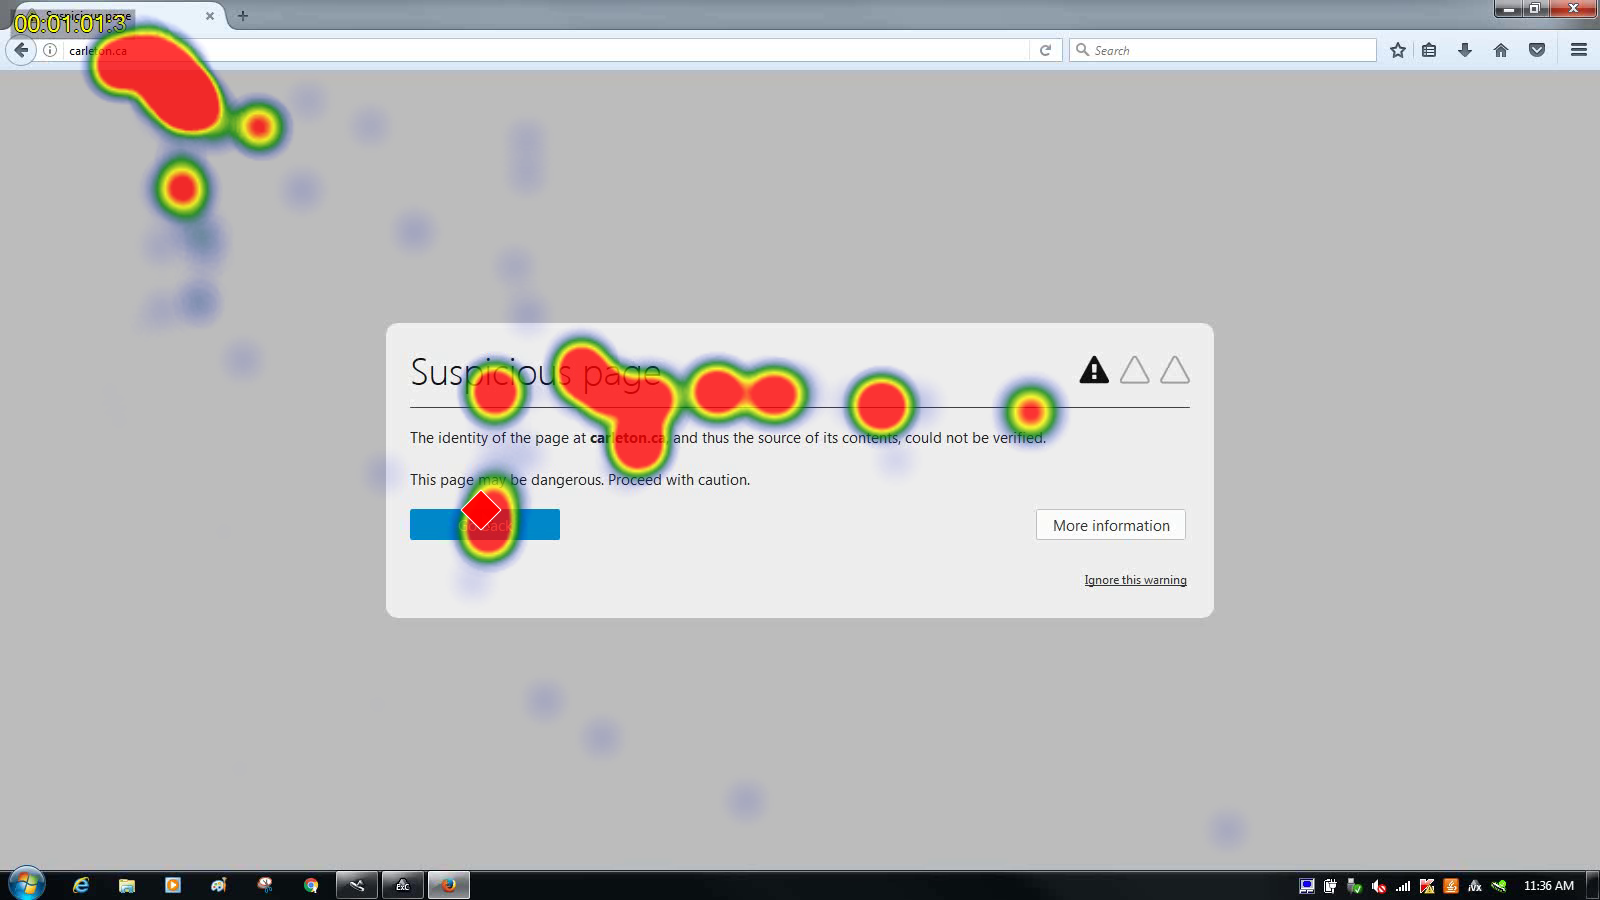
\includegraphics[width=\textwidth]{Figures/Heat-Map-P1-Low}
	\decoRule
	\caption[Phase 1 example heatmap]{A heat map of a participant viewing a low severity warning in phase 1 of the study. Note the focus on the title and lack of attention to the body. The participant also looked at the domain name (both in the URL bar and in the message body). The red diamond indicates a click.}
	\label{fig:Heatmap-Phase1}
\end{figure}

Eye tracking data shows that some participants checked the URL bar (presumably to verify that the destination URL was correct; a heatmap of one such instance is pictured in figure \ref{fig:Heatmap-Phase1}). This is typically a good security practice, but unfortunately a matching URL indicated total security for some. As Almuhimedi et al. \cite{almuhimedi2014reputation} found in a previous study, many participants trusted the website they were trying to visit and therefore felt it was probably still safe to continue regardless of the fact that a warning was displayed (e.g., ``I knew that the page was trustworthy'', ``Sometimes warning messages will appear on sites I know are safe/secure'', ``Ignored because I was accessing a trusted site''). Conversely, other participants understood that a warning on a trusted page is concerning, with remarks such as ``I was going to a page I've been to before so I automatically knew something was wrong'' and ``[An] email provider would never have such an issue so getting such a warning is very suspicious'', but these participants were in the minority. We attribute this divide in mindsets to a lack of (or improper) security education. The participants who trusted the email website appear to associate risk online purely with dangerous websites and do not consider the possibility of compromised servers (i.e., no harm can come when visiting a ``good'' website). Indeed, one participant stated that they had ``visited [the] webpage before without ill effects'', assuming that since nothing harmful had happened on the trusted site in the past, nothing harmful would happen in the future. There was little awareness of the fact that widely-used websites are large targets for attackers.

\subsection{Warning Comprehension}
Many participants ignored the warning in phase 1 relatively quickly. In a subsequent questionnaire, they were asked to identify the type of warning they had seen. Only participants who were exposed to an SSL certificate warning were able to recall it just moments later (with the exception of the low severity tiered warning). All other message types (malware, phishing, and unwanted software) could not be recalled, and many participants identified them as SSL certificate warnings as well. We suspect that most participants were guessing, with those in the SSL group happening to guess correctly. Again, this is consistent with habituation effects. Participants were likely over-exposed to SSL certificate warnings and consequently associated all browser warnings with certificate errors. Interestingly, at the conclusion of the study, all participants reported that the first message was either ``very easy'', ``easy'', or ``neutral'' in terms of clarity. We attribute this to faded memory and a lack of attention to the messages to begin with. 12 of our 20 participants changed their rating of the warning message in phase 1 when asked again at the conclusion of the study (after viewing all of the warnings in phase 2).


\section{Phase 2}

\subsection{Warning Adherence}
In phase 2 of the study we found that participants were significantly more likely to adhere to our high severity tiered messages and significantly less likely to adhere to our low and medium severity warnings (compared to the Firefox control warnings). This is explained by participants learning our warning cues over time. Eye tracker data shows that most participants initially looked at almost all aspects of the warnings but stopped reading the whole body of the messages (sometimes skimming it) after a while. A heatmap of one instance of this behaviour is pictured in figure \ref{fig:Heatmap-Phase2}. We observed a consistent pattern in the majority of participants: they would look at the warning title, then the imagery (if present), then the button corresponding to their decision, and finally they would click the button. They also began comparing warning messages to each other as the study went on. One noted that a low severity tiered warning ``only had one of three caution symbols filled in''. Another responded ``[This message is] not as intimidating as the red [one(s)]''.

Additionally, although every warning in phase 2 was unique (types did not repeat, severity levels did) many participants incorrectly stated at some point that they had seen a warning message previously in the study (e.g., ``I have already seen that warning multiple times and I have chosen to ignore it'', ``Repeated viewings of same warning, and I am ignoring them'', ``Same [warning] as before''). This behaviour indicates that they were only looking at warning features which changed with severity. Participants became habituated after learning the ``correct'' risk level and accompanying decision for a given warning tier. Those that ignored or adhered to a warning of a given severity level generally performed the same action for different messages of the same level, replicating the results of previous studies \cite{felt2015improving, sunshine2009crying}. 

\begin{figure}[!htb]
	\centering
	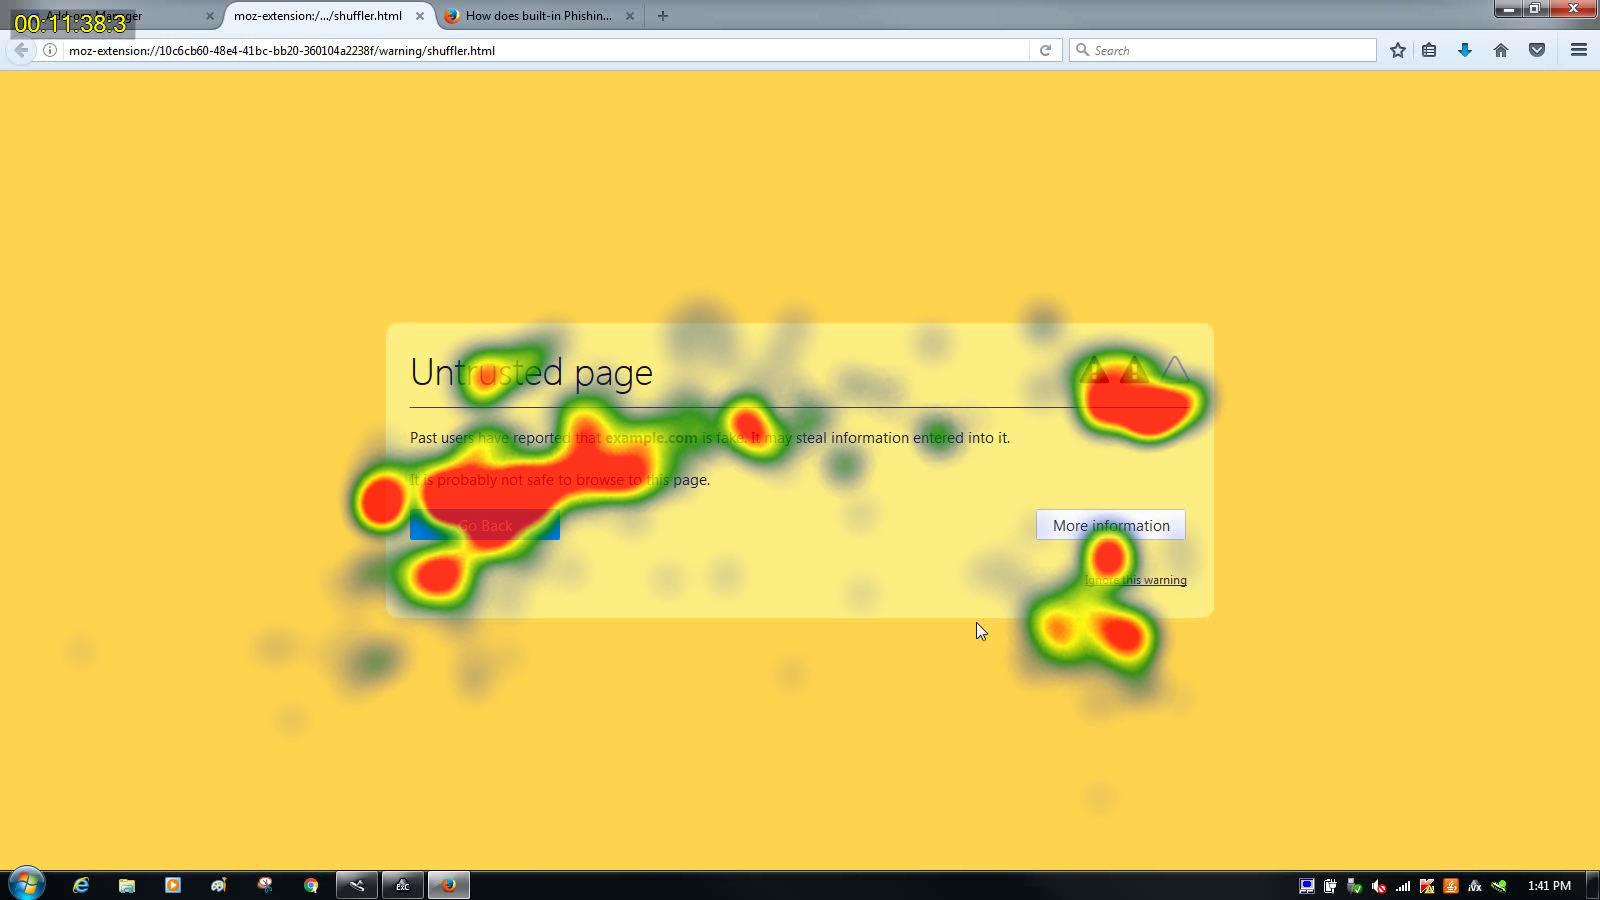
\includegraphics[width=\textwidth]{Figures/Heat-Map-P2-Medium}
	\decoRule
	\caption[Phase 2 example heatmap]{A heat map of a participant viewing a medium severity warning in phase 2 of the study. Note the attention paid to the warning icons and area surrounding the ``go back'' button.}
	\label{fig:Heatmap-Phase2}
\end{figure}

Participants had some other problematic ideas with regards to web security. For both the control and tiered warning messages, they vastly underestimated the difficulty in detecting and/or avoiding malware. Some participants who ignored warning messages responded that their reason for doing so was because they trusted either themselves or antivirus software to make the right decision with regards to security. For example, some responses to ignored ``unwanted software page'' warnings were ``I feel like the website is something my antivirus software can take care of'' and ``I [will] just make sure not to download anything and not to click suspicious-looking buttons''. Participants were unaware of attacks such as drive-by downloads and browser exploitation, which are admittedly unlikely to be known by the uninitiated.

\subsection{Severity Rating}
After learning our warning cues, participants consistently rated our high severity warnings as more severe than the control messages. We attribute this in part to a good warning design which allowed them to more easily gauge severity. As mentioned above, many participants compared our tiered messages to each other when explaining their perceptions of the severity.

The presence of the lower tiers of warnings likely also impacted severity ratings. Observing a high severity warning directly after a low severity one, for example, is a much more dramatic difference than seeing two consecutive high severity warnings. If true, this would mean that real-world users would need to be made aware of the other types of messages in order for high severity ones to be more effective. Unfortunately, the low and medium severity warnings had significantly \emph{lower} adherence rates than Firefox's default warnings. Adherence rates would have to be lowered in some cases in order to improve in others. A possible solution to this problem is to explain the different warning messages to users on first use of the browser and only show the lower tiers of messages when a threat is uncertain (a troubling tradeoff). On the other hand, it could be the case that the potential improved warning perception is not significant, and that the high severity warnings are effective on their own. However, this needs to be investigated further.

\subsection{Reaction Time}
Participants took significantly less time to make a decision when presented with a tiered message than they did with a control message. This is true for both warnings they ignored and those they adhered to. In section \ref{Results}, we suggested that this could mean either our messages conveyed severity in an easier to understand manner or that they appeared less important and were thereby more quickly dismissed. Given the improved results in adherence and severity perception, it is reasonable to conclude that the speed difference was due to a more easily identifiable level of danger.

\subsection{Warning Design}
\subsubsection{Colour}
Participant responses validated our assumptions about colour associations and our reliance on colour as a primary visual cue. On the post-study questionnaire, 80\% of participants rated colour as the most important factor for them in determining severity of messages (note that some participants tied colour with another feature of the messages). 18 of 20 rated red as the most severe colour, followed by yellow, and then grey. One rated yellow and grey as equal, and another rated grey as more severe than yellow due to a feeling of uncertainty. The responses are in line with our design goals and in phase 2 of the study our red messages were adhered to the most -- a result in agreement with the findings of Braun et al. \cite{braun1994color}.

\subsubsection{Body Text}
On the post-study questionnaire, 20\% of participants rated wording as the most important factor for them in determining severity of messages (note that some participants tied wording with another feature of the messages). Our severe messages featured concrete examples of real-world consequences such as passwords or financial information being stolen. Our goal was to make the harm more relatable and immanent, which participants picked up on (noting, for example ``I didn't like the possibility of other people seeing my passwords/private information'').

The threat description present in some of our tiered messages mentioned that other users had reported the fictional page. Participant reactions to these warnings were split. Some found the fact that another real human had reported the page more alarming, making the threat seem more legitimate. However, in others this resulted in a \emph{decreased} perception of the risk (e.g., ``It was reported to have security issues by other users, but not necessarily for me''). It is also possible that our brief (low severity) warnings caused participants to look into them more and be more cautious. One participant stated, ``somehow a more vague message made me more apprehensive than some of the others''.

At the conclusion of the study, the 20 participants were asked to identify all warning types which were presented to them in phase 2 from a list of possibilities (which included 4 warning types that were not present in the study). 15 participants remembered viewing SSL certificate warnings, 17 remembered malware warnings, 18 remembered phishing warnings, and 16 remembered unwanted software warnings. 6 participants chose one or more of the incorrect options. Although participants largely focused on the other aspects of the warnings, it appears that the body was succinct enough to effectively convey the warning type nevertheless in most cases.

\subsubsection{Imagery}
As mentioned above, eye tracking data shows that participants made frequent use of the triangular warning icons in assessing the danger of our tiered warning messages (e.g., some specifically cited low/high numbers of the icons for ignoring/adhering to a warning). Indeed, many were able to accurately describe the meaning of the imagery on the post-study questionnaire (e.g., ``More triangles meant it was more dangerous and risky to continue'', ``They were a rating system for the severity of the warning because they're similar to warning signs for the road'', ``The more icons there were the less likely I was to proceed with the page''). Additionally, one participant mentioned that they were dyslexic and that ``it was much easier to understand [the warnings] based on image and colour''. We therefore conclude that supplementing the other severity indicators with this information was very successful.

\pagebreak
\subsubsection{``More Information'' Text}
While not many participants clicked the ``more information'' button on our tiered warnings, those that did tended to read the entire threat explanation (shown in the eye tracking data). On the other hand, participants who clicked to find out more about a Firefox warning were discouraged. Doing so brought them to another page which contained information about 3 different types of warnings with no indication of which one the user came from. The approach taken by Mozilla proved to be very unusable. The page either confused participants or contained too much text to be deemed worth reading. Participants responded on the questionnaire that ``for the website to direct me to another website is kind of unusual to me'' and ``I didn't want to read the explicit explanation on the second page''. We suggest that warning designers provide a quick, clear, and easy way for users to find out more about the specific threat of interest without taking them out of current situation.


\section{Limitations}
As mentioned before, there were not enough participants to make statistically supported conclusions regarding the behaviour in phase 1 of the study. After viewing the first message, the surprise is ruined and therefore participants cannot be shown any more warnings. Possible solutions for this are to recruit more participants (if possible) or have participants perform benign tasks in between warning messages with the time between varying. The latter option, however, would be difficult to implement effectively without quickly alerting most participants to the true nature of the study. The data we did gather during phase 1 was nevertheless valuable for observing realistic behaviour and habituation effects, as well as reproducing the results of previous studies. Additionally, no participants claimed to be aware of the deception, meaning we were able to successfully structure the study so as to receive more genuine reactions.

Some participants in phase 1 noted that they felt they \emph{needed} to access their email inboxes when in fact we made a point to stress the opposite. According to these participants, having this mindset influenced their decision (it caused them to ignore the warning). In addition to the problem of few samples, this further taints our phase 1 data.

Another possible source of influence is the participants' awareness of the study's ethics approval. Participants might have assumed that their information was safe since the study was approved by the university's Research Ethics Board (noted on all recruitment material and the consent form). This would lessen any notion of risk in phase 1.

In phase 2 of the study, participants were fully aware of the purpose of the study and knew that they would be asked questions about the warning messages they were presented with. It is reasonable to assume that having this information in mind caused them to pay more attention to the warnings. The results obtained in phase 2 may therefore not be very generalizable to everyday browsing.

Next, as noted above, several participants' decisions in phase 2 were impacted by mention in some of the warning messages of other real-world users reporting danger. We did not explicitly plan the use of this wording other than purposefully excluding it from the low severity tiered messages. The presence of it in some messages at the medium and high tiers but not others may have affected participant behaviour and thus our results.

Finally, participants often compared our tiered warning messages to each other (e.g., ``there was only one warning symbol out of three that were coloured in'') and learned their relative severity ratings. Participants' perception of the high severity tiered message is likely predicated on the existence of the low and medium severity tiered warnings. Further experimentation is needed to determine whether or not the difference in perception of the high severity warning on its own is significant and how much it affects adherence.
